
\documentclass[11pt]{article}
\usepackage[utf8]{inputenc}
\usepackage[a4paper, total={165mm, 216mm}]{geometry}

% package for language setting ---------------------------------------------
\usepackage[english]{babel}

% package used for paragraph formatting ------------------------------------
\usepackage{parskip, fancyhdr, url, rotating, appendix}

% packages used for images -------------------------------------------------
\usepackage{graphicx}
\graphicspath{{images/}}
\usepackage{float}

% packages used for references ---------------------------------------------
\usepackage{xcolor} % Load this for color definitions
\usepackage{natbib}
\usepackage{hyperref}
\hypersetup{
    colorlinks = true,
    linkcolor = gray,
    citecolor = gray,
    urlcolor  = gray
}
\bibliographystyle{apalike}

% package for eqations -----------------------------------------------------
\usepackage{amsmath}


% package used for degree symbol -------------------------------------------
\usepackage{textcomp, gensymb}


% packages used for tables -------------------------------------------------
\usepackage{multirow, makecell, booktabs,longtable,array,ragged2e, graphicx, chngpage, afterpage, geometry, color}

% package used for caption -----------------------------------------------
\usepackage[format=hang,font=small,labelfont=bf]{caption}
\captionsetup{justification   = raggedright,
              singlelinecheck = false}
              

% no indentation
\setlength\parindent{0pt}

% set running headings on each page
% https://www.overleaf.com/learn/latex/Headers_and_footers
\pagestyle{headings}
\pagestyle{fancy}
\rhead{\theauthor}
\lhead{\thetitle}
\cfoot{\thepage}

% 2500 - 3000 words
\begin{document}

%\BgThispage
% --- edit ---
\author{B. Fábryová} % author
\title{Impact of forest landscape dynamics on seeds in naturally regenerating tropical forests} % title
\newcommand\subtitle{Report}
\newcommand\supervisor{Dr. I. Hordijk} % supervisor
\newcommand\secondsupervisor{Dr. D. Masiliunas} % second supervisor
\newcommand\studentnumber{1176870} % student number
\date{2025} % date

% --- do not edit ---
\makeatletter 
\let\thetitle\@title
\let\theauthor\@author
\let\thedate\@date
\makeatother

\begin{titlepage}
	\centering
    \vspace*{.5 cm}
    
\includegraphics[height = 3.8 cm]{Proposal/graphics/WUR_logo}\\[1.0 cm]
    \textsc{\LARGE WAGENINGEN UNIVERSITY \& RESEARCH}\\
    \textsc{\small Droevendaalsesteeg 4, Wageningen, The Netherlands}\\[0.5 cm]
	\textsc{\large Master's of Geo-Information Science}\\[2.0 cm]
	\textsc{\Large MSc Thesis}\\[0.5 cm]
	\rule{\linewidth}{0.2 mm} \\[0.4 cm]
	{\huge \bfseries \thetitle}\\[0.4 cm]
	{\Large \bfseries \subtitle} \\
	\rule{\linewidth}{0.2 mm} \\[1.5 cm]
	
	\begin{minipage}[t]{0.4\textwidth}
		\begin{flushleft} \large
			\emph{Author:}\\
			\theauthor\\[0.5 cm]
			\emph{Supervisor:}\\
			\supervisor\\[0.5 cm] 
			\emph{Second supervisor:}\\
			\secondsupervisor\\
		\end{flushleft}
	\end{minipage}~
	\begin{minipage}[t]{0.4\textwidth}
		\begin{flushright} \large
			\emph{Student Number:} \\
			\studentnumber
		\end{flushright}
	\end{minipage}\\[1.32 cm]
	{\large \thedate}\\
 
	\vfill
	
\end{titlepage}

\newpage
\tableofcontents

\newpage
\section{Introduction}


% INTRODUCTION
% •	Start at a broader societal or scientific context (e.g., climate change, sustainability challenges) and then narrow down to the main topic of the thesis. 
% •	Include descriptions of:
    % •	what are general ways (or opportunities) to tackle certain issues (e.g., need accurate information to respond/mitigate climate change)
    % •	What kind of scientific data and methods can be used? 
    % •	What further possibilities are there? (e.g., new satellite data, new technical advancements)
    % •	Avoid including the thesis research goals here (there is a separate section – section 3)
% •	At least 5 peer-reviewed references ( preferably not older than 10 years)
% •	Page indication:1

% RESEARCH NEEDS
% • This section is generally more specific compared to the previous section focusing on questions like what needs to be researched and what the research gaps are. For example, there are new opportunities (e.g. new tools or data sources), but further study is needed to evaluate their use/value.  
% • This section is not to confuse with “societal needs”, it only focuses on research needs. The societal needs/context is already tackled in the introduction section. 
% • The research needs descriptions are often linked with the research questions of the proposal. In other words, with this thesis research, by answering the research questions, your work will contribute to bridging the current research gap. 
% • This section can be combined with the introduction section, but the main content needs to be present. 
% • At least 10 peer-reviewed references (preferably not older than 10 years) 
% • page indication: 1

% RESEARCH AIM AND RESEARCH QUESTIONS
% •	Apply the SMART principle for the research objective (Specific, Measurable, Attainable, Relevant and Time-bound)
% •	Research questions should be linked to research needs/gaps
% •	Avoid closed questions with “yes/no” answer and questions such as “how to” or “how can”. The latter questions involve certain choices in methods. Hence the obtained results can be only specific to the chosen steps/methods. 
% •	To define a clear research question, it is useful to imagine the expected answer to the questions and also the form of the answer: e.g., map, lists, tables, and figures. 
% •	See more explanations on research questions here (Brightspace discovery course for scientific reading and writing)

% General
Tropical forests are the world's key ecosystems, providing habitat for a wide diversity of species, supporting local livelihoods, and playing an integral role in global ecological cycles such as carbon sequestration, water regulation, and nutrient cycling \citep{bormaCarbonContributionsSouth2022}. They host approximately two-thirds of the world's flora and fauna, making them essential habitats for global biodiversity \citep{mulatuBiodiversityMonitoringChanging2017}. Tropical ecosystems are not only crucial for wildlife, but also for local livelihoods of millions of people who rely on their resources for food, medicine, and income \citep{bormaCarbonContributionsSouth2022}. Despite their importance, over half of the tropical forests have been deforested and converted into other land use types, with agriculture being the most common, leading to loss of these vital ecosystem services \citep{chazdonNaturalRegenerationTool2016, arroyo-rodriguezMultipleSuccessionalPathways2017}. Given the growing pressure on tropical forests, natural forest regeneration presents a promising solution for ecological restoration \citep{hordijkLandUseHistory2024}. Natural forest regeneration is a spontaneous recovery process during which native tree species colonize land following human-induced or natural disturbances \citep{crouzeillesEcologicalRestorationSuccess2017}. This process is particularly significant in tropical regions, where intensive agriculture practices often lead to resource depletion and thus to land abandonment. Over time, vegetation and soil can recover, resulting in the formation of a secondary forest \citep{chazdonSecondGrowthPromise2014}. However, the success of natural regeneration is strongly influenced by seed inflow, which relies on the availability of seed sources and dispersers in the surrounding landscape. Seed inflow is therefore dependent on the spatial factors, such as the degree of landscape fragmentation and the proximity to surrounding forest \citep{arroyo-rodriguezMultipleSuccessionalPathways2017}. Although substantial research has been published on the importance of the surrounding forest for seed inflow during natural forest regeneration \citep{dentUnitingNicheDifferentiation2021, arroyo-rodriguezMultipleSuccessionalPathways2017, v.h.safarLandscapeOpennessHas2022}, there is an existing knowledge gap on how the surrounding forest impacts seed inflow in wet versus dry tropical forests. Therefore, this study aims to investigate the effects of forest landscape cover, connectivity, and age on a fundamental component of natural forest regeneration: the seed, and compare these effects between wet and dry tropical secondary forests.

% On secondary succession
In ecological terms, the transition from herbaceous to woody plants dominated vegetation is known as secondary succession - a directional change in ecosystem attributes over time following a disturbance. Unlike primary succession, secondary succession benefits from land legacies such as well-established soils and the presence of propagules, the reproductive units of plants \citep{poorterSuccessionalTheories2023}. % here a potential to elaborate on the history of succession theories development
Successional theory has evolved over time, with 
key frameworks proposed by \citet{pickettHierarchicalConsiderationCauses1987} and \citet{poorterComprehensiveFrameworkVegetation2024}, identifying three main successional mechanisms: (1) site availability, (2) species availability, and (3) species performance. Site availability depends on the type, intensity and duration of a disturbance, which in turn impacts seed bank and remnant vegetation \citep{poorterComprehensiveFrameworkVegetation2024}. Species availability is regulated by propagules that remain at the site after the disturbance and those dispersed into the site \citep{gleasonIndividualisticConceptPlant1926, dentUnitingNicheDifferentiation2021}. Finally, species performance is determined by species traits, biotic interactions, and the abiotic environment \citep{poorterComprehensiveFrameworkVegetation2024}. 

% On seeds
Among these, species availability often has the strongest influence on the speed and the direction of the first phase of succession \citep{poorterSuccessionalTheories2023, dentUnitingNicheDifferentiation2021}. However, due to an agricultural land history, remnant propagules such as seedbanks and resprouts might be limited or depleted. Thus, leaving the species availability mechanism dependent on propagules dispersed into the site, also known as seed rain. The diversity and abundance of seeds in the seed rain are thereafter important factors for secondary succession. They are determined by biotic dispersers such as birds and mammals and abiotic dispersers such as wind and water \citep{poorterComprehensiveFrameworkVegetation2024}. The dominant mode of dispersal might vary during different stages of succession. Early successional stages are most commonly characterized by wind, birds and bats dispersal, whereas later successional stages, when seed abundance increases are more commonly characterized by larger mammals dispersal \citep{dentUnitingNicheDifferentiation2021}. Moreover, dispersal mode can also vary between wet and dry tropical forest. In dry tropical forest, seeds are more likely to be smaller and dispersed by wind, whereas in wet tropical forest, seeds tend to be covered in fleshy fruit and dispersed by frugivores \citep{}. 
The mode of seed dispersal and therefore the abundance and diversity of seeds is, however, in turn dependent on the landscape surrounding the regenerating forest site. 

%Wind dispersed species are especially common in degraded landscapes, however animal dispersed species are necessary for driving a diverse succession 

% On landscape factors
The landscape factors such as the age of the forest, the forest cover and the forest connectivity play a critical role in the seed abundance, diversity and distribution. Moreover, the surrounding forest functions as a seed source and as a habitat for seed dispersers and pollinators \citep{hordijkLandUseHistory2024, arroyo-rodriguezMultipleSuccessionalPathways2017}. The distance to an established forest has a strong influence on the seed dispersed to the re-establishing site, given that most seeds are distributed over short distances \citep{chazdonSecondGrowthPromise2014}. This leads to a higher abundance of seeds in sites that are in a close proximity to an established forest \citep{hordijkLandUseHistory2024}. Additionally, it is not only the presence of surrounding forest, but also the degree of connectivity between the existent forest patches that has a strong influence on the regenerating forest site. Well connected forest patches positively impact abundance of animal dispersed seeds, whereas more distanced forest patches have usually higher abundance of wind dispersed seeds \citep{dentUnitingNicheDifferentiation2021}.

%Landscapes
%at one extreme: landscape dominated by forested matrices are mainly determined %by local variation of environmental factors since seed abundance is relatively %high, whereas landscape dominated by various land use types will be mainly %determined by factors operating at landscape and regional scale, especially %those which affect production, dispersal, and predating of propagules

% gap
While these mechanisms are broadly applicable, the factors shaping the successional pathway might vary substantially between ecosystems. For instance, in tropical forests, the process differs between dry and wet tropical forest. In wet tropical forest, succession is more dependent on the landscape connectivity and the availability of seed dispersers, as most tree species rely on animals for dispersal. In contrast, tropical dry forest is dominated by wind-dispersed species \citep{hordijkLandUseHistory2024, lohbeckSuccessionalChangesFunctional2013}. Although substantial research has been published on the mechanisms of secondary succession and to its related landscape factors, few studies have investigated the detailed effects of their impact on tree seed diversity and dispersal comparing dry and wet tropical forest ecosystems. Understanding the mechanisms of secondary succession broadens our knowledge on how ecosystems respond to a disturbance. This is particularly important in the age of Anthropocene during which global land use and climate change cause severe disruptions in the ecosystems.  Therefore, the aim of this study is to understand how forest landscape factors affect seed diversity and dispersal in a dry and wet tropical forest during early succession. Given this, the following research question has been identified: \textit{How does forest age, cover and connectivity affect seed abundance, richness and dispersal mode in dry and wet secondary tropical forests during early succession?} By understanding the dynamics present in secondary succession, we can design and implement more effective ecosystem restoration strategies \citep{poorterSuccessionalTheories2023}.

%The terms investigated in this research are defined as following:\\\\
%\textit{Forest landscape factor terms.}\\
%\textbf{Forest age:} the number of years since a forest's establishment.\\
%\textbf{Forest cover:} spatial extent covered with trees.\\
%\textbf{Forest connectivity:} the degree of agglomerations between forest patches.\\
%\\
%\textit{Seed diversity and dispersal terms.} \\
%\textbf{Seed richness:} measure of the number of different seed species.\\
%\textbf{Seed evenness:} measure of the relative abundance of different seed species.\\
%\textbf{Seed dispersal mode:} the mechanisms by which a seed is moved from a source to an establishment site.\\

It is hypothesized that seed richness and evenness will increase with forest age in both dry and wet tropical forests (Fig. \ref{fig:cf}). Species richness will increase due to the arrival of new species over time and species evenness will increase due to decline in dominants pioneer species as early successional species are gradually replaced by later successional species \citep{poorterSuccessionalTheories2023, chazdonNaturalRegenerationTool2016}. Forest age is expected to have positive impact on biotic dispersal, however, negative impact on abiotic dispersal as abiotic dispersal is mostly present during early stages of succession. It is further hypothesized that forest connectivity and cover will have positive impact on seed richness and evenness as they facilitate larger and more varied seed pool. Moreover, it is hypothesized they have a negative impact on seed abiotic dispersal due to lower ability of wind dispersed seeds to travel further. In contrast, forest connectivity is hypothesized to have positive impact on biotically dispersed seeds as connectivity favors seed dispersers movement. 

% something that might be related to the age of the forest -> "This confirms that early-successional species invest in many small seeds that can travel large distances (e.g., by wind), whereas late-successional species invest in fruits that attract biotic dispersers to allow directional dispersal" (Lohbeck)

% Natural forest regeneration is an effective tool for various ecological restoration efforts such as climate change mitigation, biodiversity conservation, or soil health restoration \citep{hordijkLandUseHistory2024}. 
% It supports global ambitions such as the restoration of 3.5 million $km^2$ of degraded land \citep{holl2017restoring} and aligns with the UN Decade on Ecosystem Restoration, which aims to reach land degradation neutrality by 2030 \citep{waltham2020decade}. 

\begin{figure}[]
\begin{center}
		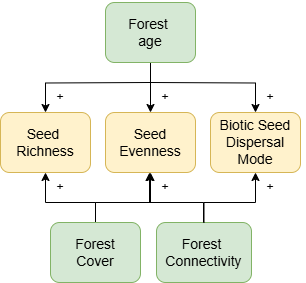
\includegraphics[]{Proposal/graphics/contextual_framework.drawio.png}
	\caption{Conceptual framework}
\label{fig:cf}
\end{center}
\end{figure}

\section{Methodology}

% METHODOLOGY
% •	Study area description, if any
% •	Justify certain choices of methods and datasets
% •	Be clear on what will be investigated using what metrics. For example, the research will study the uptake of solar panel installation for different provinces by comparing the number of households that have solar panel installations since 2015. 
% •	Be clear on how to validate the results and using what metrics. For example, assess the accuracy of detecting solar panels using overall accuracy, user’s accuracy, precision, etc.,
% •	Clearly describe any ground truth or reference data, e.g., how to access and how/what to collect
% •	page indication: 2 

\subsection{Study sites}
This research will be carried out in dry tropical forest at an elevation of 90-120~m a.s.l. located in the area of Nizanda (16°39' N, 95°00' W), Mexican province of Oaxaca and in the wet tropical forest at an elevation of 115-300~m a.s.l. located in the area of Loma Bonita (16°01' N, 90°55'), Mexican province of Chiapas. 

The dry tropical forest has a mean annual temperature of 27.7°C and seasonal rainfall with a mean annual precipitation of 900~mm where 90\% of the total annual rainfall occurs between May and October. It is characterized as dry tropical deciduous forest \citep{hordijkLandUseHistory2024}. 

The wet forest has a mean annual temperature of 24°C and a mean annual precipitation of 3000~mm with a relative dry season between February and April accounting for less than 10\% of the total annual rainfall. The vegetation varies between semideciduous and lowland tropical rain forest \citep{hordijkLandUseHistory2024}.

There are twenty (25~m x 25~m) plots established in both the dry and wet tropical forest. These plots were established on recently abandoned (0-10 months following abandonment) pasture or agricultural land by the PANTROP project in March 2020 \citep{hordijkLandUseHistory2024}. If needed, plots were fenced off to prevent grazing. 


\subsection{Seeds}
To evaluate the seed diversity and dispersal mode in both forest sites (wet and dry), four seed traps were established in each plot. In the dry forest, the seed traps were rectangular with the dimensions of 50~cm x 50~cm and in the wet tropical forest, the seed traps were circular with the diameter of 1~m. The seed traps were positioned 6~m from the plot's edge in each corner of the plots. The seeds were collected monthly for a duration of one year in 2023. The content of the four traps was combined into one sample per plot.

Subsequently, the collected seeds were separated into groups of unique species. Each group of unique seed species  was counted by the number of individuals, weighted by the total weight per group and identified by species. The identification of seed species was performed with a seed catalog provided by Universidad Nacional Autonóma de México (UNAM) and with the support of research assistant Marina Beatriz Hernandez Mendez, an expert in tropical wet forest seed identification, and ..., an expert in tropical dry forest seed identification. 

\subsubsection{Seed attributes}
% define how to calculate the seed attributes?
In order to evaluate seed richness, evenness and dispersal mode. The mode of dispersal is based on literature.

% For this research, a fieldwork will be conducted in the dry tropical forest in Nizanda, Mexico. 
% Unfortunately, it is not possible to conduct fieldwork in the wet tropical forest in Loma Bonita due to the political situation at place. However, data on wet tropical forest and historical data on both sites will be retrieved from the PANTROP project database to be able to analyse and compare wet and dry tropical forest.

\subsection{Forest Landscape Factors}
To evaluate the forest landscape factors, remote sensing techniques will be employed, as historical field data is scarce and interview-based data can be unreliable and difficult to obtain \citep{decuyperContinuousMonitoringForest2022}. In this context, the forest landscape factors are defined as follows: 1) \textit{forest age}: the number of years a forest remained undisturbed, up to a maximum of 25 years (the limit of satellite imagery availability), 2) \textit{forest cover}: the percentage of surrounding forest within a given radius, 3) \textit{forest connectivity}: the percentage of patches adjacent to each other. 
These factors will be assessed using the Anomaly Vegetation Change Detection (AVOCADO) algorithm, which is based on the R package "npphen". AVOCADO is designed to detect forest disturbance and regrowth based on satellite imagery in a semi-automated and continuous manner. It utilizes all available data without requiring outlier removal \citep{decuyperContinuousMonitoringForest2022}. As a time series algorithm, AVOCADO analyzes more than two satellite images to detect change. Compared to change bi-temporal difference methods or supervised image classification, time series approaches offer greater precision in detecting small-scale forest changes by capturing the dynamic behavior of vegetation over time. 

The AVOCADO algorithm uses a reference vegetation from a nearby pixel known to have remained undisturbed throughout the time series. This reference pixel will be selected with the help of an expert with a long-term field experience in the area. 

The input to the AVOCADO algorithn will be Landsat derived Normalized Difference Moisture Index (NDMI) image. Landsat is selected due to its long historical archive. While Landsat spatial resolution (30m) is sometimes considered a hindrance compared to its temporal resolution, this is not a significant limitation for the current study, as the resolution is comparable to the spatial scale of the investigated forest plots (25m). NDMI, derived from Lndsat's near-infrared and shortwave infrared bands, is used as it is sensitive to changes in vegetation moisture and canopy structure. This makes NDMI particularly effective for detecting forest disturbances and regrowth.

The output of the algorithm is a raster map with an indication of the year since the last disturbance. This map will be used for a further evaluation of the forest age, forest cover, and forest connectivity using the landscapemetric or the lconnect package in R \citep{mestreLconnectPackageVersatile2023, hesselbarthLandscapemetricsOpensourceTool2019}. The satellite imagery used will be Landsat NDMI images.
\citep{gore}

The evaluation will be performed in R software \citep{R}.

\subsection{Statistical analysis}
To investigate how seed richness, evenness and seed dipersal mode are affected by forest age, cover and connectivity, a Linear Mixed Model will be performed. The model will be evaluated using $R^2$, RMSE and AIC.

 

\section{Time Schedule}

% TIME SCHEDULE
% •	Plan the time schedule considering the main methods or research questions
% •	Indicate if working part-time or other engagements such as a teaching assistant job, holidays, etc.
% •	Consider also the main milestones such as the proposal, midterm presentation, research questions, validation and writing /finalising
% •	Preferable to use a Gantt Chart, project planning timeline, network diagram, Kanban board or any other visual aid for project management
% •	page indication: 0.5 

This section elaborates on the proposed time frame for this MSc thesis research. The start date of this research is 01.02.2025 and the predicted end date is 30.09.2025. For a detailed overview, see Table \ref{tab:timeschedule}.

\begin{table}[h]
\captionof{table}\\{\textit{Proposed time schedule for the MSc Thesis Research}}\\

\begin{tabular}{lll}\hline
\multicolumn{1}{c}{\textbf{When}} & \multicolumn{1}{c}{\textbf{What}}   & \multicolumn{1}{c}{\textbf{Where}} \\\hline
01/02/2025 - 14/02/2025           & Proposal writing + presentation     & Wageningen (NL)                    \\
16/02/2025 - 02/03/2025           & Fieldwork in Nizanda                & Nizanda, Oxaca (MX)                \\
03/03/2025 - 06/04/2025           & Labwork in Morelia                  & Morelia, Michoacan (MX)            \\
07/04/2025 - 20/04/2025           & Time off                 &           \\
21/04/2025 - 18/07/2025           & Data processing + analysis          & Wagenigen (NL)                     \\
19/04/2025 - 31/08/2025           & Time off                 &           \\

01/09/2025 - 30/09/2025           & Report writing + final presentation & Wageningen (NL)\\\hline                 
\end{tabular}\label{tab:timeschedule}
\end{table}

This is a proposed and expected time frame for the research. However, this research contains fieldwork, which might result in an occurrence of unforeseen circumstance due to which an adaptation of the schedule might be needed. 

\section{Feasibility}

% FEASIBILITY
% •	What could be potential risks and how you will mitigate these? Examples are computing time, access to data, knowledge gap etc.
% •	page indication: 0.5 

In case of inability to collect data in the field, a historical data from the PANTROP database will be used. Additionally, to avoid computational issues, a remote server, Papaya, will be used.

\section{AI Statement}
The use of generative AI in this article is limited to correcting grammar and \LaTeX{} syntax.

\newpage
\bibliography{references}

\end{document}